% report_31_01_2018.tex
% Omkar H. Ramachandran
% omkar.ramachandran@colorado.edu
%
% Documentation for hemispheric dependence in the Fermi Pass 8 data
%

\documentclass[english]{article}
\usepackage[T1]{fontenc}
\usepackage[latin9]{inputenc}
\usepackage{geometry}
\geometry{verbose,tmargin=1.5in,bmargin=1.5in,lmargin=1.5in,rmargin=1.5in}
\usepackage{babel}
\newcommand{\GeV}{\,{\rm GeV}}
\usepackage{graphicx}
\graphicspath{{./plots/}}
\usepackage{hyperref}
\usepackage{listings}
\usepackage{color}

\lstdefinestyle{custompy}{
  belowcaptionskip=1\baselineskip,
  breaklines=true,
  frame=L,
  xleftmargin=\parindent,
  language=Python,
  showstringspaces=false,
  basicstyle=\footnotesize\ttfamily,
  keywordstyle=\bfseries\color{green},
  commentstyle=\itshape\color{red},
  identifierstyle=\color{black},
  stringstyle=\color{blue},
}

\lstset{escapechar=@,style=custompy}

\begin{document}
\title{Prelab 3 : Filters}
\author{Omkar H. Ramachandran}

\maketitle

Note: I do not have Mathematica installed on my work laptop - which is an 8+ 
year old Lenovo flex 10. Thus, I have completed all the prelab activities in
Python and have written it up in \LaTeX. In addition, all the code present in
this document is available on my 
\href{https://github.com/ShadowWarden/electronics}{Github repository}

\section{Low and High-pass filters}
\subsection{Define Python functions to calculate the cutoff}
For both low-pass and high-pass RC filters, the cut off frequency is the same:
$$ f_{C} = \frac{1}{2\pi RC} $$
The code to return $f_{C}$ given $R$ and $C$ is as follows:
\begin{lstlisting}
def compute_cutoff_RC(R,C):
    """ Returns cutoff frequency for an RC filter """
    return 1./(2*np.pi*R*C)
\end{lstlisting}
This function can simply be called as follows:
\begin{lstlisting}
R = 10e3
C = 1e-9
Fc = compute_cutoff_RC(R,C)
\end{lstlisting}
Evaluating this function for the values in the schematic yeilds
$F_c = 15.9154\, kHz$

\subsection{Bode plots for each filter}
A bode plot is simply a plot of the transfer function $H(\omega)$ on log
-log axes. We know that, for a low-pass filter,
$$ |H(\omega)| = \frac{1}{\sqrt{1+(RC\omega)^{2}}} $$
The code to generate these plots is as follows:
\begin{lstlisting}
def plot_bode_RC(R,C,omega_min,omega_max,flag):
    """ Plots the bode function between the given limits. The flag
    decides whether the transfer function used is for the high-pass 
    or low-pass filter"""
    Nomega = 1000
    H = np.zeros(Nomega)
    omega = np.linspace(np.log(omega_min),np.log(omega_max),Nomega)
    if(flag == 0):
        # Low pass
        H = 1./np.sqrt(1+(R*C*np.exp(omega))**2)
    elif(flag == 1):
        # High pass
        H = (R*C*np.exp(omega))/np.sqrt(1+(R*C*np.exp(omega))**2)
    plt.figure(1)
    plt.plot(omega,H,'r-.',label='$R = %.2f\, K\Omega, C = %.2f\, pF$' % (R/1e3,C/1e-9))
    plt.xlabel(r"$\ln\omega$")
    plt.ylabel(r"$H(\omega)$")
    plt.legend()
    plt.grid()
    plt.draw()
    return H
\end{lstlisting}
To call one of these functions, one simply needs to execute the following:
\begin{lstlisting}
R = 10000
C = 10**(-9)
omega_min = 1.0
omega_max = 10**8
# For low pass, execute the following:
H = plot_bode_RC(R,C,omega_min,omega_max,0)
# And for high pass,
H = plot_bode_RC(R,C,omega_min,omega_max,1)
plt.show()
\end{lstlisting}
The program will automatically generate and label plots that look as in Figure 1:
\begin{figure}
	\centering
	\label{fig:boderc}
	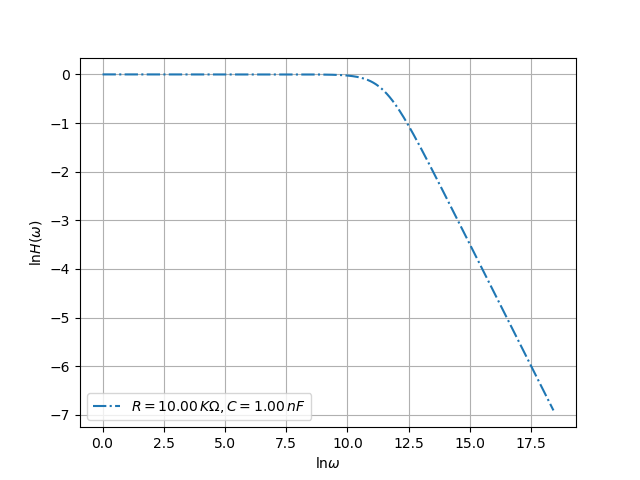
\includegraphics[scale=0.4]{low_pass_question.png}
	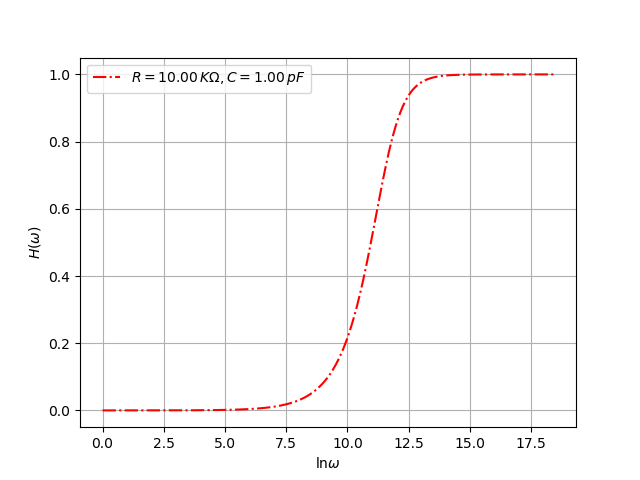
\includegraphics[scale=0.4]{high_pass_question.png}
	\caption{(left) Plot of low-pass and (right) high-pass bode curves for $R=10\,K\Omega$ and $C=1000\,pF$}
\end{figure}

\subsection{Generate mock data}
The following code snippet chooses 50 points uniformly on the log $x$ scale 
and then plots them in the appropriate place. Note: This function must be 
called only \textbf{after} the main curve plotting function has already been
called
\begin{lstlisting}
def generate_mock_RC(R,C,omega_min,omega_max,flag):
    """ Generates lots of mock data that follows bode curve """
    Npoints = 50
    Nomega = 1000
    omega = np.linspace(np.log(omega_min),np.log(omega_max),Nomega)
    P_omega = (1.0*np.ones(Nomega))/Nomega
    plt.figure(1)
    for i in range(Npoints):
        omega_choice = np.random.choice(omega,p=P_omega)
        if(flag == 0):
            # Low pass
            H = 1./np.sqrt(1+(R*C*np.exp(omega_choice))**2)
        elif(flag == 1):
            # High pass
            H = (R*C*np.exp(omega_choice))/np.sqrt(1+(R*C*np.exp(omega_choice))**2)
        plt.plot(omega_choice,H,'bo')
        plt.draw()
\end{lstlisting}
Running this function creates plots as in Figure 2
\begin{figure}
	\centering
	\label{fig:mockrc}
	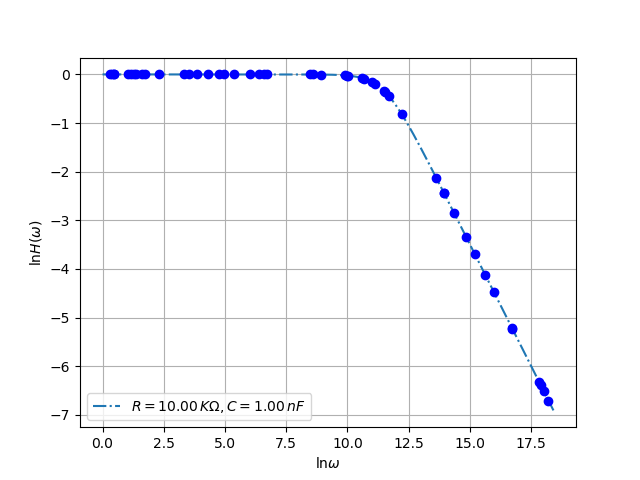
\includegraphics[scale=0.4]{mock_low.png}
	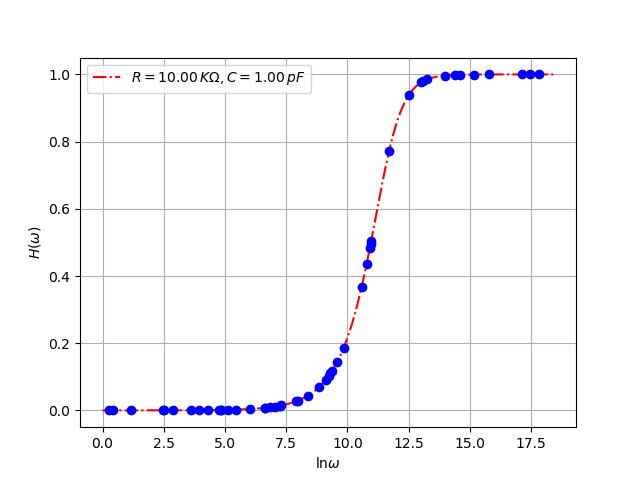
\includegraphics[scale=0.4]{mock_high.png}
	\caption{(left) Plot of low-pass and (right) high-pass bode curves for $R=10\,K\Omega$ and $C=1000\,pF$.
	Each curve has further been populated with fake data points}
\end{figure}

\section{Band-pass Filters}
\subsection{Define functions that calculate $f_0$}
For the band-pass filter, the required parameters are defined as follows:
$$ f_0 = \frac{1}{2\pi\sqrt{LC}} $$
$$ Q = 2\pi f_0 RC $$
$$ Z_0 = 2\pi f_0 L $$
Thus, the code to compute these is as follows:
\begin{lstlisting}
def compute_parameters_BP(R,L,C):
    """ Returns the required parameters for a band-pass filter """
    f0 = 1/(2*np.pi*np.sqrt(L)*np.sqrt(C))
    Q = 2*np.pi*f0*R*C
    Z0 = 2*np.pi*f0*L
    return np.array([f0,Q,Z0])
\end{lstlisting}
To run this, we simply use the following:
\begin{lstlisting}
R = 10e3
L = 10e-3
C = 1e-8
f0,Q,Z0 = compute_parameters_BP(R,L,C)
\end{lstlisting}
For the values in the schematic, the output from the code is $f_0 =15.9154\, kHz$, 
$Q =9.999$ and $Z_0 =999.9\, \Omega$

\subsection{Bode plots for band-pass filters}
The code to generate bode plots for the band pass filter is as follows:
\begin{lstlisting}
def plot_bode_BP(R,L,C,omega_min,omega_max):
    """ Plots the bode function between the given limits. The flag
    decides whether the transfer function used is for the high-pass 
    or low-pass filter"""
    Nomega = 1000
    H = np.zeros(Nomega)
    omega = np.linspace(np.log(omega_min),np.log(omega_max),Nomega)
    H = R/np.sqrt(R**2+(np.exp(omega)*L-1/(np.exp(omega)*C))**2)
    
    plt.figure(1)
    plt.plot(omega,H,'r-.',label='$R = %.2f\, K\Omega, C = %.2f\, pF$' % (R/1e3,C/1e-9))
    plt.xlabel(r"$\ln\omega$")
    plt.ylabel(r"$H(\omega)$")
    plt.legend()
    plt.grid()
    plt.draw()
    return H
\end{lstlisting}
It generates plots as in Figure 3.
\begin{figure}
	\centering
	\label{fig:bandpass}
	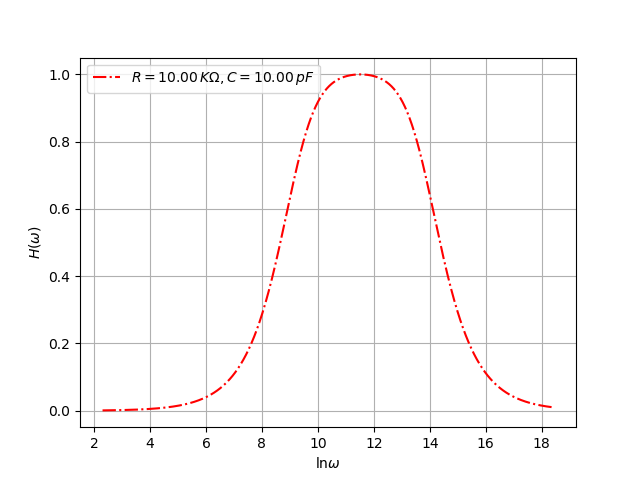
\includegraphics[scale=0.4]{band_pass.png}
	\caption{Plot of band-pass bode curves for $R=10\,K\Omega$ and $C=1000\,pF$}
\end{figure}

\subsection{Mock Data for the Band Pass filter}
The code to generate mock data on the bode-curve is as follows:
\begin{lstlisting}
def generate_mock_BP(R,L,C,omega_min,omega_max):
    """ Generates lots of mock data that follows bode curve """
    Npoints = 50
    Nomega = 1000
    omega = np.linspace(np.log(omega_min),np.log(omega_max),Nomega)
    P_omega = (1.0*np.ones(Nomega))/Nomega
    plt.figure(1)
    for i in range(Npoints):
        omega_choice = np.random.choice(omega,p=P_omega)
        H = R/np.sqrt(R**2+(np.exp(omega_choice)*L-1/(np.exp(omega_choice)*C))**2)
        plt.plot(omega_choice,H,'bo')
        plt.draw()
\end{lstlisting}
Once again, it must only be called after the curve is already plotted, since
it inherits the axial labeling. Once called, it generates values as in Figure 4
\begin{figure}
	\centering
	\label{fig:mockbp}
	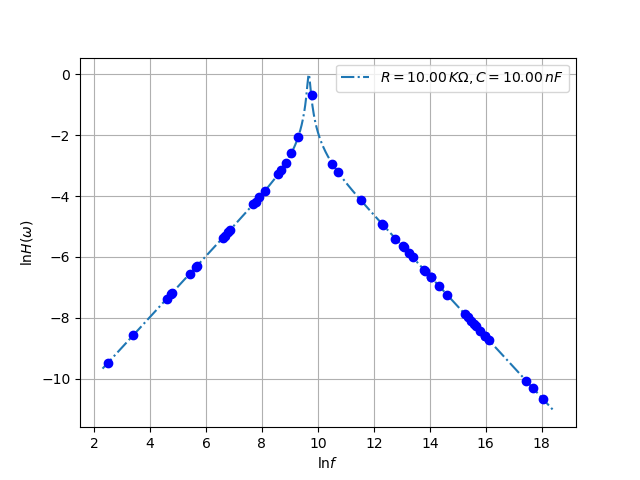
\includegraphics[scale=0.4]{band_pass_mock.png}
	\caption{Plot of band-pass bode curves for $R=10\,K\Omega$ and $C=1000\,pF$.
	Each curve has further been populated with fake data points}
\end{figure}

\section{Lab Activities}
\begin{itemize}
	\item Step 6 looks to be the hardest, especially point b, given that
		we need to use the prelab model in conjunction with the oscilloscope measurement
	\item I'm still not completely sure as to why we needed to generate the mock data.
\end{itemize}

\end{document}
